% ****** Start of file apssamp.tex ******
%
%   This file is part of the APS files in the REVTeX 4.1 distribution.
%   Version 4.1r of REVTeX, August 2010
%
%   Copyright (c) 2009, 2010 The American Physical Society.
%
%   See the REVTeX 4 README file for restrictions and more information.
%
% TeX'ing this file requires that you have AMS-LaTeX 2.0 installed
% as well as the rest of the prerequisites for REVTeX 4.1
%
% See the REVTeX 4 README file
% It also requires running BibTeX. The commands are as follows:
%
%  1)  latex apssamp.tex
%  2)  bibtex apssamp
%  3)  latex apssamp.tex
%  4)  latex apssamp.tex
%
\documentclass[%
 reprint,
%superscriptaddress,
%groupedaddress,
%unsortedaddress,
%runinaddress,
%frontmatterverbose, 
%preprint,
%showpacs,preprintnumbers,
%nofootinbib,
%nobibnotes,
%bibnotes,
 amsmath,amssymb,
 aps,
%pra,
%prb,
%rmp,
%prstab,
%prstper,
%floatfix,
]{revtex4-1}

\usepackage{graphicx}% Include figure files
\usepackage{dcolumn}% Align table columns on decimal point
\usepackage{bm}% bold math
\usepackage{comment}
\usepackage{amsmath}
\usepackage[hidelinks]{hyperref}% add hypertext capabilities
%\usepackage[mathlines]{lineno}% Enable numbering of text and display math
%\linenumbers\relax % Commence numbering lines

%%\usepackage[showframe,%Uncomment any one of the following lines to test 
%%scale=0.7, marginratio={1:1, 2:3}, ignoreall,% default settings
%%text={7in,10in},centering,
%%margin=1.5in,
%%total={6.5in,8.75in}, top=1.2in, left=0.9in, includefoot,
%%height=10in,a5paper,hmargin={3cm,0.8in},
%%]{geometry}

\begin{document}

%\preprint{APS/123-QED}

\title{Adiabatic Quantum Computation \\ Physics 506 Term Paper}% Force line breaks with \\

\author{Adam Mills}
\email{armills@princeton.edu}
\affiliation{Princeton University}

\date{\today}% It is always \today, today,
             %  but any date may be explicitly specified

\begin{abstract}
	The circuit, or gate, model of quantum computation is largely regarded as the ``standard'' model of quantum computation. The circuit model evolves the Hilbert space as it operates on an initial state via a prescribed series of unitary operations. This series of unitary operations is analogous to the logical gate operations performed in a classical computer. Adiabatic quantum computation attempts to solve a computational problem by evolving the quantum processor from the ground state of some initial Hamiltonian that is simple to some final Hamiltonian that encodes the solution of the original problem in the ground state. The adiabatic method is universal and robust, and as a result has attracted a lot of theoretical and experimental interest. This paper explores some of the basic theory of adiabatic quantum computation and adiabatic algorithms that are known to provide a proven quantum speedup. Following, a specific experimental example of factoring a number is used to provide some context for the theory.
\end{abstract}

\maketitle

%\tableofcontents

%===================================================

\section{Introduction}

   Most anyone who has studied quantum computation (QC) is familiar with the circuit, or gate, model of QC\cite{Deutsch73}. It considered the ``standard'' model of QC and is arguably the most intuitive form of quantum computation as it closely resembles classical computing. One starts with the qubits of the quantum processor in a given state and then performs a series of unitary operations on them in the form of gates according to a prescribed algorithm. In the end, the final state of the processor encodes the solution to the problem. 

   There is, however, an entirely different approach to quantum computation that does not employ quantum gates. Adiabatic Quantum Computation (AQC) attempts to solve a computational problem by encoding the solution to the problem in the ground state of some problem Hamiltonian, $H_p$, and adiabatically transitioning to this Hamiltonian from some initial Hamiltonian, $H_0$\cite{RevModPhys.90.015002}. Thus, we have a time-dependent Hamiltonian that performs a smooth interpolation between $H_0$ and $H_p$ of the form 
	\begin{equation}
		H(t) = (1-s(t))H_0 + s(t)H_p, 
		\label{eq:Ht}
	\end{equation}
where the schedule, $s(t)$, is defined such that
	\begin{center}
		$s(0) = 0, \hspace{1cm} s(T) = 1,$
	\end{center}
and $T$ is the total evolution time. The whole system then evolves according to the Schr{\"o}dinger equation
 	\begin{center}
		$i\dfrac{d}{dt}\vert\psi(t)\rangle = H(t)\vert\psi\rangle$.
	\end{center}
	
   The idea is that the initial Hamiltonian is easy to prepare in the ground state while the final Hamiltonian is more difficult. As the adiabatic algorithm slowly evolves the Hamiltonian of the quantum processor from $H_0$ into the problem Hamiltonian, $H_p$, the adiabatic theorem guarantees that at the end of the transition the system will still be in the ground state barring any disturbances. Thus, the final state will represent the encoded solution to the problem. 

   In this overview of AQC, I discuss some of the theory behind adiabatic quantum computation in Section~\ref{sec:A} before presenting several adiabatic algorithms. I then present a specific experimental example in Section~\ref{sec:B} where AQC is used to factor a number. The paper concludes with a short term outlook for AQC.
   
   \section{Adiabatic Computation}\label{sec:A}
   
   This section examines the appeal of using adiabatic transitions to perform computation as well as some of the known adiabatic algorithms. It is reasonable to ask why one would not just prepare the final Hamiltonian in a cold environment and wait for thermal relaxation to bring the system down to the ground state. The problem with this approach is that some hard optimization problems pose a more complex solution space that contain local minima. In such cases, the computer may get stuck in these states from which downward transitions are unlikely, causing equilibration time to grow exponentially large in the number of bits being used to run the algorithm.
   
   Adiabatic quantum computation is a rather robust form of QC against the typical problems that plague the gate model, in part due to these potentially hard to make transitions, i.e., decohering. The circuit model relies on actively controlling the qubits from one step to the next and has to fight and correct for dephasing, decoherence, and unitary control errors along the way. In AQC, the phase of the ground state does not influence the results of the algorithm, so dephasing in the energy eigenbasis has no impact. The adiabatic method is also only efficient if the minimum energy gap is reasonably large, so the method is robust against decoherence under typical operational conditions\cite{Childs2001}. AQC does not rely on performing unitary gates throughout the algorithm, but it is susceptible to errors in implementing the time-dependent Hamiltonian, $H(t) + K(t)$. Childs \textit{et al.} showed that this error in the implementation, $K(t)$, can actually be reasonably large as long as it is slowly varying and has small initial and final values. It is also true that $K(t)$ can rapidly fluctuate as long as the characteristic frequency of the fluctuations is large compared to the energy scale of $H(t)$.
   
   The robustness of AQC is attractive, but the most important question that has to be answered is whether or not AQC provides a quantum speedup over classical algorithms. A quantum speedup can be classified in several ways\cite{RevModPhys.90.015002}. To borrow from Albash \textit{et al.}, a ``provable'' quantum speedup is backed by a proof that no classical algorithm can outperform the quantum algorithm. A ``strong'' quantum speedup compares the quantum algorithm to the best classical algorithm, explicitly known or not, but is not backed by any solid proof. A ``quantum speedup'' is a speedup against the best available classical algorithm, but could be superseded by a better classical algorithm. Finally, a ``limited'' quantum speedup is a speedup by comparison to a classical algorithm that uses the same algorithmic approach, but on classical hardware.
   
   Of these, the most interesting class of speedups are the provable quantum speedups as they guarantee that the effort put into implementing a reliable quantum algorithm will yield an improvement over the classical implementations. For AQC, there are several algorithms that offer a provable quantum speedup, three of which are briefly presented below.
   
   \begin{itemize}
   	\item The adiabatic Grover search algorithm is the AQC parallel of the circuit model Grover search algorithm. The goal of the algorithm is to find a marked item, or multiple marked items, in an unsorted database of \textit{N} items with as few queries to the database as possible. A classical algorithm must query the database until the marked item is found. As a result, the number of queries will scale linearly in \textit{N}. On the other hand, the adiabatic Grover algorithm scales as $\sqrt{N}$ offering a quadratic speedup over classical algorithms.
   \item The adiabatic Deutsch-Jozsa algorithm is another AQC parallel of an existing circuit model algorithm. The Deutsch-Jozsa problem is to determine whether or not a function, $f: \lbrace0,1\rbrace^n \longmapsto \lbrace0,1\rbrace$, is balanced or constant using as few calls to the function as possible. Classical algorithms require $2^{n-1} + 1$ queries to $f$ in the worst case since a balanced function could return a constant answer for the first $2^{n-1}$ queries. Just like the quantum circuit model Deutsch-Jozsa algorithm, the adiabatic run time is $O(1)$.
   \item The adiabatic Bernstein-Vazirani algorithm solves the problem of locating an unknown binary string $ a \in \lbrace0,1\rbrace^n  $ with as few queries to the oracle as possible. The circuit model and adiabatic model both offer a solution that runs with $O(1)$ queries. Both offering a polynomial quantum speedup over classical algorithms that require $n$ queries.
   \end{itemize}
   
   These three examples illuminate an important relation between the two different quantum computation methods. Each adiabatic algorithm had a quantum circuit model counterpart that scaled the same way. Although three examples is nothing to draw a definitive conclusion from, it is no coincidence that this correlation exists. In fact, adiabatic quantum computation is proven to be equivalent, up to polynomial overhead, to the circuit model and thus universal\cite{Aharanov2007}. 
   
   The equivalence between the AQC and gate model QC can be stated more formally borrowing a definition from Albash \textit{et al.}: ``A time-dependent Hamiltonian $H(t), t\in [0,t_{f}]$ is universal for AQC if, given an arbitrary quantum circuit $U$ operating on an arbitrary initial state $\vert\psi\rangle$ of $n$ p-state particles and having depth $L$, the ground state of $H(t_f)$ is equal to $U\vert\psi\rangle$ with probability greater than $\epsilon>0$, the number of particles $H(t)$ operates on is $poly(n) \forall t$, and $t_f = poly(n,L)$.\cite{RevModPhys.90.015002}''

   This definition stipulates that the final state of the circuit, $U\vert\psi\rangle$, is equal to the final ground state of $H(t)$, ensuring that the circuit model and adiabatic model of computation have the same output. It is important to note that as a result of their equivalence, quantum circuits can simulate adiabatic computations\cite{Farhi2000} and vice versa\cite{Aharanov2007}.
   
   There are a few different constructions of universal AQC based on simulating a quantum circuit that is described by a sequence of $L$ one-qubit or two-qubit unitary gates $U_1 , U_2 , ... U_L$. One such construction is presented here to provide some context. Fermionic ground state quantum computation is a method of AQC that executes an $n$-qubit quantum circuit of depth $L$ by spatially encoding the entire temporal trajectory of the circuit, from input to output, in the ground state of a two-dimensional array of quantum dots\cite{Mizel2001}. The system is constructed with $L+1$ columns and $2n$ rows, where the rows correspond to the $\vert 0 \rangle$ and $\vert 1 \rangle$ basis states of the qubit. For each unitary gate, a Hamiltonian term is introduced with off-diagonal terms that represent hopping or tunneling of the electron between neighboring sites and unitary terms that act on the electron's spin. This Hamiltonian is tuned in by a parameter, $s \in [0,1]$, from some initially prepared ground state at $s=0$ when every electron is frozen in place and no tunneling occurs to full realization of all of the quantum gates, $U^{(1)}_{q,l}$, when $s=1$.
   
   \section{Experimental Discussion}\label{sec:B}
   
   This section details an experimental realization of an adiabatic factoring algorithm. A much more basic system than the previously mentioned 2-dimensional array has recently been used to factorize the number 35\cite{Xu2017}. Xu \textit{et al.} demonstrated AQC using a single spin system realized in a nitrogen-vacancy (NV) center in diamond. NV centers are attractive as good quantum processors and sensors at room temperature\cite{DOHERTY20131}. They have long coherence times, allow for fast resonant spin manipulation, and are easy to initialize and read-out using laser illumination. In this example, solving the problem begins by constructing a multiplication table, for example Table~\ref{tab:binmult}, from which one can create a set of equations that will be mapped onto the problem Hamiltonian.
   
   The problem Hamiltonian is constructed bitwise by directly mapping the binary variables to operators on qubits\cite{Xu2012}. In this example, we have the general Hamiltonian 
	\begin{equation}	
	H_p = \left( \hat{p} + \hat{q} -1 -2\hat{z_{12}} \right)^2 .
	\end{equation}
This comes from looking at the second column where $p$ and $q$ sum to 1 and $z_{12}$ is carried. So the equation that is mapped onto the general problem Hamiltonian is $p+q=1+2z_{12}$.

\begin{table}[h]
\begin{flushleft}
\begin{tabular}{ p{1.7cm}  p{1cm} p{1cm} p{1cm} p{1cm} p{1cm} p{1cm}} \hline\hline
 & \textit{$2^5$}  & \textit{$2^4$}  & \textit{$2^3$}
& \textit{$2^2$}   & \textit{$2^1$} & \textit{$2^0$} \\ \hline

x &\hspace{0.1cm} &\hspace{0.1cm} &\hspace{0.1cm} &1 &p &1 \\ 

y &\hspace{0.1cm} &\hspace{0.1cm} &\hspace{0.1cm} &1 &q &1 \\ 

\hspace{0.1cm} &\hspace{0.1cm} &\hspace{0.1cm} &\hspace{0.1cm} &1 &p &1 \\ 

\hspace{0.1cm} &\hspace{0.1cm} &\hspace{0.1cm} &q  &qp &q &\hspace{0.1cm} \\ 

\hspace{0.1cm} &\hspace{0.1cm} &1 &p  &1 &\hspace{0.1cm} &\hspace{0.1cm} \\ 

Carries &$z_{45}$ &$z_{34}$ &$z_{23}$ &$z_{12}$ &\hspace{0.1cm} &\hspace{0.1cm} \\ 

\hspace{0.1cm} &$z_{35}$ &$z_{24}$ &\hspace{0.1cm}  &\hspace{0.1cm} &\hspace{0.1cm} &\hspace{0.1cm} \\ 

$x \times y = 35$ &1 &0 &0 &0 &1 &1 \\ 
\hline
\end{tabular}
\end{flushleft}
\caption{Binary multiplication table for $ 5 \times 7 = 35 $. The top row represents the significance of each bit. x and y are the multipliers. $z_{ij}$ is the carry bit from the \textit{i}th bit to the \textit{j}th bit, and the row in the bottom is the number that we want to factor\cite{Xu2017}.
}
\label{tab:binmult}
\end{table}

	
	\begin{figure}[h]
	%% try any of the variations to take more control of the figure placement
	% h = here
	% \begin{figure}[h] 
	% H = HERE
	% \begin{figure}[H]
	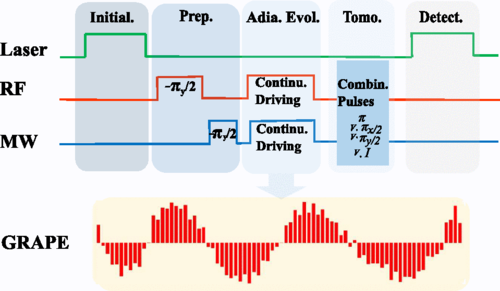
\includegraphics[scale=0.49]{Fig2XuEtAl}
	\caption{	
		The pulse sequence of the adiabatic factorization process. Under the condition that the external magnetic field is near 510 G aligned with the NV axis, the 532 nm laser pulse initializes both the electron spin and the $^{14}$N nuclear spin. To prepare the initial state to $\Psi_i = \dfrac{1}{2}\left(\vert 0 \rangle - \vert 1 \rangle   \right)\left(\vert 0 \rangle - \vert 1 \rangle   \right)$, RF and MW pulses are applied successively. The above panel shows that the adiabatic evolution can be realized through continuously applying the RF and MW pulses. In the actual experiment, evolution of the state is driven by the optimal control pulse instead. In the lower panel is the optimal control pulse applied on the nuclear spin. (Figure and caption taken from Xu \textit{et al.}\cite{Xu2017})
	}
	\label{fig:pulse}
	\end{figure}


	 Now the problem can be simplified a little more by noting that the variables are binary. This reduces the equation to $p+q=1$, as $z_{12}$ must be equal to 0.	 
	 
	  Under this mapping scheme, each operator in the problem Hamiltonian is formed as the pauli operators acting on a qubit representing each variable as follows:
	\begin{equation}
	  \hat{p} = \dfrac{I-\hat{\sigma_{1,z}}}{2} \hspace{1cm}   \hat{q} = \dfrac{I-\hat{\sigma_{2,z}}}{2}.
	\end{equation}
Using the simplification, $p+q=1$, and substituting the $\hat{p}$ and $\hat{q}$ operators for the pauli operator form, the problem is simplified to solving for the ground state of the Hamiltonian,
	
\begin{equation}
	H_p = \left( \dfrac{I-\sigma_{1,z}}{2} + \dfrac{I-\sigma_{2,z}}{2} - I\right)^2 = \left(S_z + I_z \right)^2 ,
\end{equation}
in the $\vert m_s,m_l \rangle$ basis of the NV qubit. The state encodes the solution to the problem as   $\vert p,q \rangle$.

	The initial Hamiltonian, $H_0$, is chosen to be non-commutative with $H_p$ in order to prevent energy level crossings. $H_p$ can be simplified more by dropping the identity operator and scaling it with a constant, $g_1$, in accordance with Xu \textit{et al.}. The two resulting Hamiltonians are

\begin{equation}
	H_p = g_1\left(2S_zI_z\right), \hspace{1cm} H_0 = g_2\left(S_x + I_x\right) .
\end{equation}

	The challenge now is to experimentally realize Eq.~\ref{eq:Ht}. The Hamiltonian of the NV center electron spin coupled with the $^{14}$N nuclear spin is defined as
	\begin{equation}
		H = DS_z^2 + \gamma_lB_zS_z + QI_z^2 + \gamma_nB_zI_z + \hat{S}\tilde{A}\hat{I}.
	\end{equation}

	This Hamiltonian can be transformed into the adiabatic evolution Hamiltonian, Eq.~\ref{eq:Ht}, by applying radio frequency (RF) and microwave (MW) driving\cite{Kong2016}. Using the same notation as Xu \textit{et al.}, the system Hamiltonian under rf and MW driving is
	\begin{equation}
	\begin{split}
		H^{rot}_{NV} = \left( \delta_{MW} + \delta_{RF} \right)\hat{I} + \Omega_{MW}2S_xI_z \\ - \delta_{RF}I_z + \Omega_{RF}I_x - \delta_{MW}S_z.
	\end{split}
	\label{eq:rotNV}
	\end{equation}
	
	In this system Hamiltonian, $\Omega_{MW}$ and $\Omega_{RF}$ are the Rabi frequencies while $\delta_{MW}$ and $\delta_{RF}$ are the detunings. Now set $\delta_{RF}=0$, $\Omega_{MW}\equiv s(t)g_1$, $\Omega_{RF}=-\delta_{MW}\equiv \left(1-s(t)\right)g_2$, and drop the identity operator. Eq.~\ref{eq:rotNV} becomes
	\begin{equation}
		H^{rot}_{NV} = s(t)g_12S_xI_z + \left(1-s(t)\right)g_2\left(I_x + S_z\right)
	\end{equation}
which is almost exactly Eq.~\ref{eq:Ht} using $H_p$ and $H_0$ defined for this problem. In order to complete the transformation, apply a Hadamard gate on the electron spin subspace which exchanges $S_x$ and $S_z$ and we get the Hamiltonian in the desired form
	\begin{equation}
		H^{rot}_{NV} = s(t)g_12S_zI_z + \left(1-s(t)\right)g_2\left(I_x + S_x\right).
	\end{equation}	
	
	An overview of the procedure is shown in Fig.~\ref{fig:pulse}. The NV electron spin and the nitrogen nuclear spin are polarized at the same time by applying a laser pulse at 532 nm. Then MW and RF $-\pi_y/2$ pulses ($\pi/2$ rotations about the $-y$ axis) are applied to prepare the initial state $\Psi_i = \dfrac{1}{2}\left(\vert 0 \rangle - \vert 1 \rangle   \right)\left(\vert 0 \rangle - \vert 1 \rangle   \right)$. The adiabatic process is then approximated by shaped pulses and finally tomography is performed to measure the population distribution. 

	The results of the experiment are shown in Fig.~\ref{fig:densitymatrix} as the final state density matrix. The concentration in the middle shows that the final state is most likely $\Psi_i = \dfrac{1}{\sqrt{2}}\left(\vert 01 \rangle + \vert 10 \rangle   \right)$. From this, we can extract the values of $p$ and $q$ by recalling the final state vector will be of the form $\vert pq \rangle$. The factoring problem that we were trying to solve was to find $1p1$ and $1q1$ in binary, as these are the prime factors of 35. Therefore, the algorithm yields the binary numbers $101$ and $111$ as the two prime factors which are 5 and 7 in decimal.
	
	\begin{figure}
	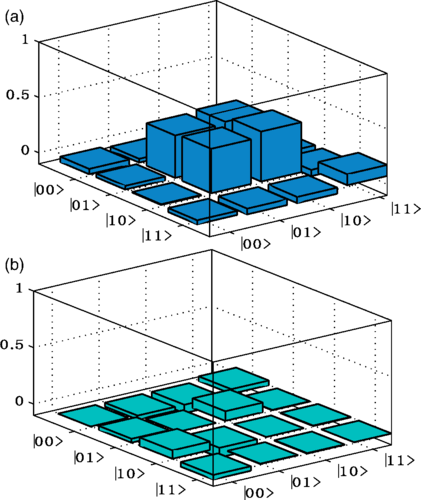
\includegraphics[scale=0.49]{Fig3XuEtAl}
	\caption{	
		Final state density matrix. (a) The real and (b) the imaginary part of the density matrix. The vertical axis shows probability while the basis of the density matrix is shown by the horizontal axes. From this final state, we can infer the answer of the factorization is $\left\lbrace p=1, q=0 \right\rbrace$ or $\left\lbrace p=0, q=1 \right\rbrace$ (Figure taken from Xu \textit{et al.}\cite{Xu2017})
	}
	\label{fig:densitymatrix}	
	\end{figure}
	
	
	This experiment exhibits the potential power of adiabatic quantum computing. Using a single qubit, the number 35 was factorized with a fidelity of about \%81 \cite{Xu2017}. The mapping scheme used to create the problem Hamiltonian scales to multiple qubits and could thus be leveraged to factor larger numbers.
	
	\section{Conclusion}
		
	The circuit model certainly seems to dominate the field of quantum computation, but the adiabatic model stands its ground. It has been rigorously proven to be equivalent to the circuit model and has also been realized experimentally in a variety of host materials. However, the field still has a lot of growing to do. Not every algorithm that offers a quantum speedup in the circuit model has a parallel AQC algorithm. There are also no known problems that can be solved with a quantum speedup using AQC that are not previously known from other models of quantum computing. The scheme also still relies on \textit{a priori} knowledge of the size and/or position of its spectral gap in order to predict an optimal adiabatic schedule for evolution of the Hamiltonian.	

	Even if with these shortcomings, adiabatic quantum computation offers a potentially more robust form of QC that does not require such extremely controlled conditions as those required by superconducting qubits or spin qubits. This may allow for larger scaling, lower costs, and improved fidelities. As these benefits only apply for the subset of problems with known adiabatic algorithms, there certainly appears to be a bright a future for theorists working to fill in the algorithmic gaps of AQC. Experimentalists have their work cut out for them in implementing currently known algorithms, improving upon fidelities, and constructing systems that can perform arbitrary computations.
%===================================================


\nocite{*} % Attaches all citations to end, regardless of whether or not they were used in text
\bibliographystyle{apl} % Get bibliography formatting
\bibliography{FinalPaperBib} % This is where your bibtex citations go

\end{document}
